\documentclass[border=4pt]{standalone}
\usepackage{amsmath,amssymb,tikz}
\usetikzlibrary{arrows.meta}
\definecolor{figB}{RGB}{31,90,166}\definecolor{figR}{RGB}{176,48,48}\definecolor{figG}{RGB}{46,125,50}\definecolor{figO}{RGB}{214,120,20}
\begin{document}
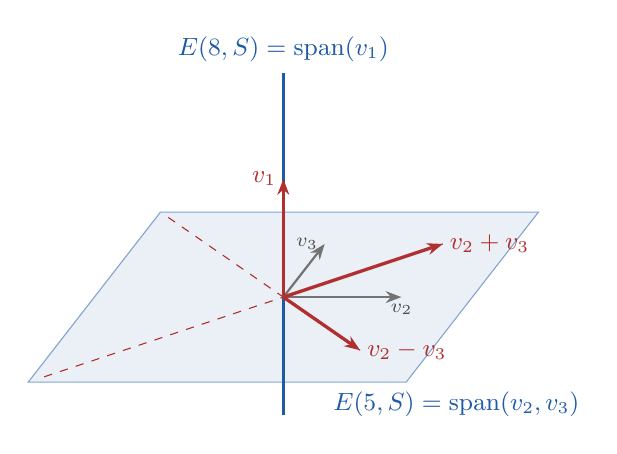
\begin{tikzpicture}[scale=1.5,>={Stealth[length=2mm]},x={(1cm,0cm)},y={(0.35cm,0.45cm)},z={(0cm,1cm)}]
% E(5,S) = span(v2,v3): a plane
\fill[figB!9] (-1.6,-1.6,0)--(1.6,-1.6,0)--(1.6,1.6,0)--(-1.6,1.6,0)--cycle;
\draw[figB!55] (-1.6,-1.6,0)--(1.6,-1.6,0)--(1.6,1.6,0)--(-1.6,1.6,0)--cycle;
\node[figB,font=\small,anchor=north west] at (0.9,-1.6,0) {$E(5,S)=\operatorname{span}(v_2,v_3)$};
% E(8,S) = span(v1): a line
\draw[very thick,figB] (0,0,-1.0)--(0,0,1.9) node[above,font=\small]{$E(8,S)=\operatorname{span}(v_1)$};
% T's eigenlines inside the plane
\draw[dashed,figR] (-1.5,-1.5,0)--(1,1,0);
\draw[dashed,figR] (-1.5,1.5,0)--(1,-1,0);
% basis of S
\draw[->,thick,black!55] (0,0,0)--(1,0,0) node[below,font=\scriptsize,black!70,inner sep=2pt]{$v_2$};
\draw[->,thick,black!55] (0,0,0)--(0,1,0) node[left,font=\scriptsize,black!70,inner sep=2pt]{$v_3$};
% common eigenvectors
\draw[->,very thick,figR] (0,0,0)--(1,1,0) node[right,font=\small,inner sep=2pt]{$v_2+v_3$};
\draw[->,very thick,figR] (0,0,0)--(1,-1,0) node[right,font=\small,inner sep=2pt]{$v_2-v_3$};
\draw[->,very thick,figR] (0,0,0)--(0,0,1) node[left,font=\small,inner sep=2pt]{$v_1$};
\end{tikzpicture}
\end{document}
